%! Author = julianmour
%! Date = 01/05/2023

\section{Preliminary Results}
We evaluated our preliminary approach on the MNIST dataset, consisting of images showing a singular digit.
The classifier's goal is to return the correct classification of a given digit. Specifically we checked the the robustness of class $c=0$.

We evaluated our algorithm against three different scenarios using three different models: a fully connected network 3X10, and two convolutional neural networks with different number of iterations during training, detailed in table~\ref{table_architectures}. For each model, noted as $D$, we defined encoded our problem definition using MIPVerify ~\cite{MIPVERIFY}, where $F_1$ is $D$ and $F_2$ is also $D$ with a slight change in a singular weight in the last layer on $D$. MIPVerify returns the bounds for the confidence and the time it took to solve. The timeout was set to 50800 seconds (14 hours, 6 min, and 40 seconds). We compared between two approaches for each model:
\begin{itemize}
    \item Solving the confidence bounds without the proposed constraints, noted as "Baseline".
    \item Solving the confidence bounds using the proposed constraints, noted as "Our approach".
\end{itemize}

\begin{table}[H]
    \centering
    \resizebox{\textwidth}{!}{
    \begin{tabular}{@{\extracolsep{\fill}}llll@{}}
        \toprule
        \makecell{Dataset} & \makecell{Name} & \makecell{Architecture}  & \makecell{Iterations during training} \\
        \midrule            
        \multirow{3}{*}{MNIST} & 3 x 10 & 3 fully-connected layers & 20 \\
                               & CNN1 & 2 convolutional (stride 4) and 2 fully-connected layers & 20 \\
                               & CNN2 & 2 convolutional (stride 4) and 2 fully-connected layers & 19 \\
        \bottomrule
    \end{tabular}
    }
    \caption{The networks used for this experience.
        \label{table_architectures}}
\end{table}

Figure~\ref{fig:3_x_10}, figure~\ref{fig:cnn0_1} and figure~\ref{fig:cnn0_2} show the gaps in the execution time for the 3X10, CNN1, and CNN2 respectively.
The preliminary results show a significant improvement of 82\% in average, across all examined models, in execution time when applying the second approach. 
\begin{figure}[ht]
  \centering
  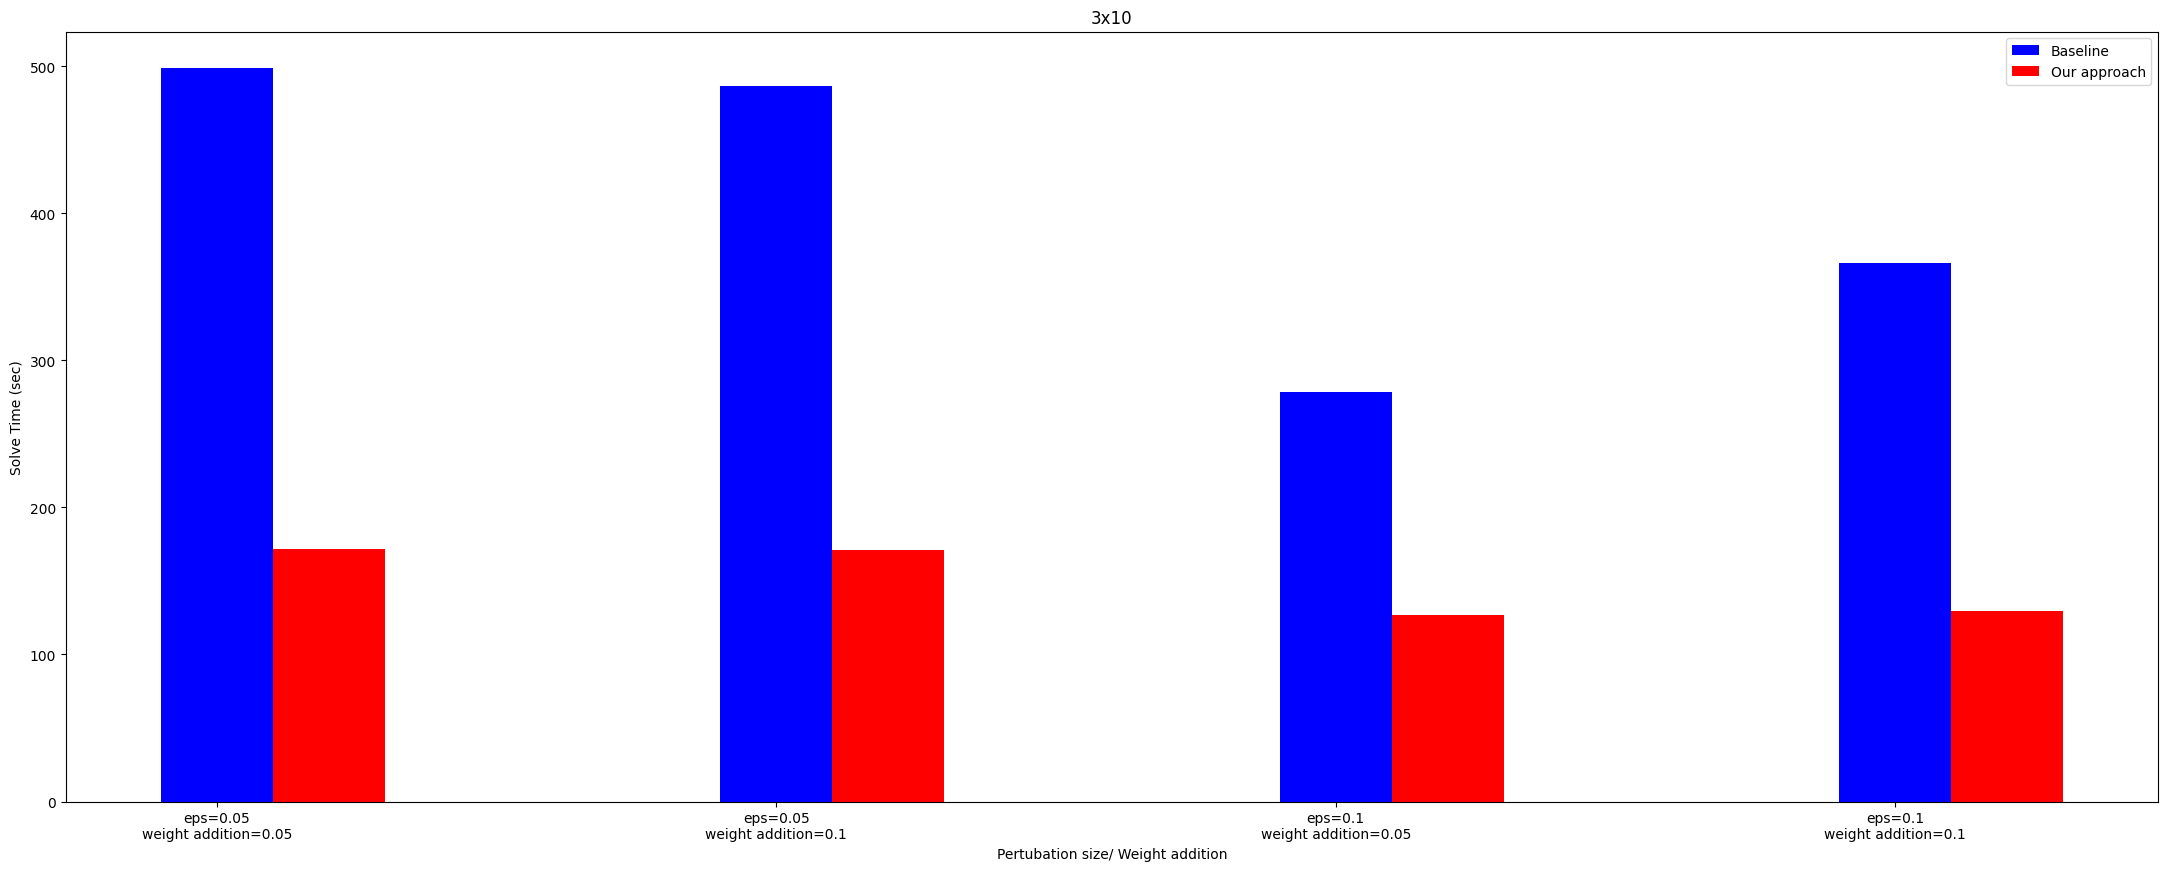
\includegraphics[width=0.95\textwidth]{3x10.png}
  \caption{The execution time of the baseline against our approach, when the model type is a fully connected network 3x10 .}
  \label{fig:3_x_10}
\end{figure}

\begin{figure}[ht]
  \centering
  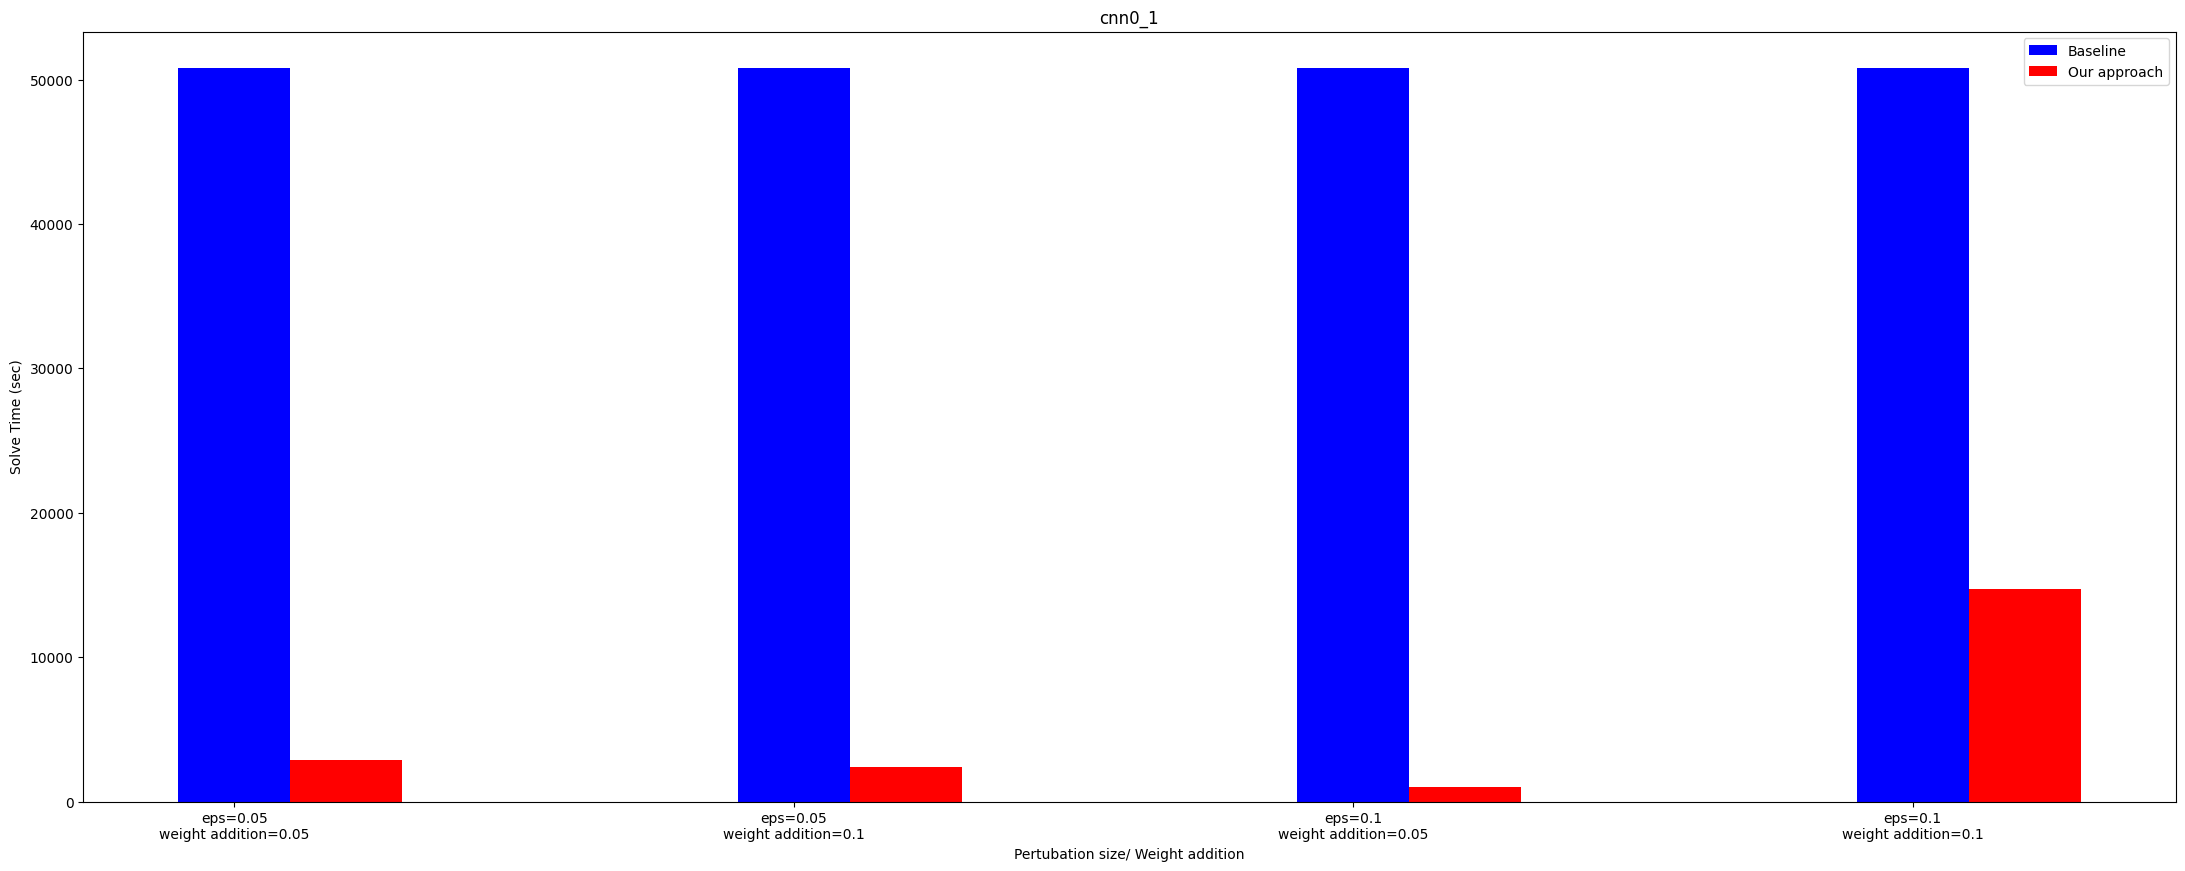
\includegraphics[width=0.95\textwidth]{cnn0_1.png}
  \caption{The execution time of the baseline against our approach, when the model type is a convolutional neural network, trained using 20 iterations .}
  \label{fig:cnn0_1}
\end{figure}

\begin{figure}[ht]
  \centering
  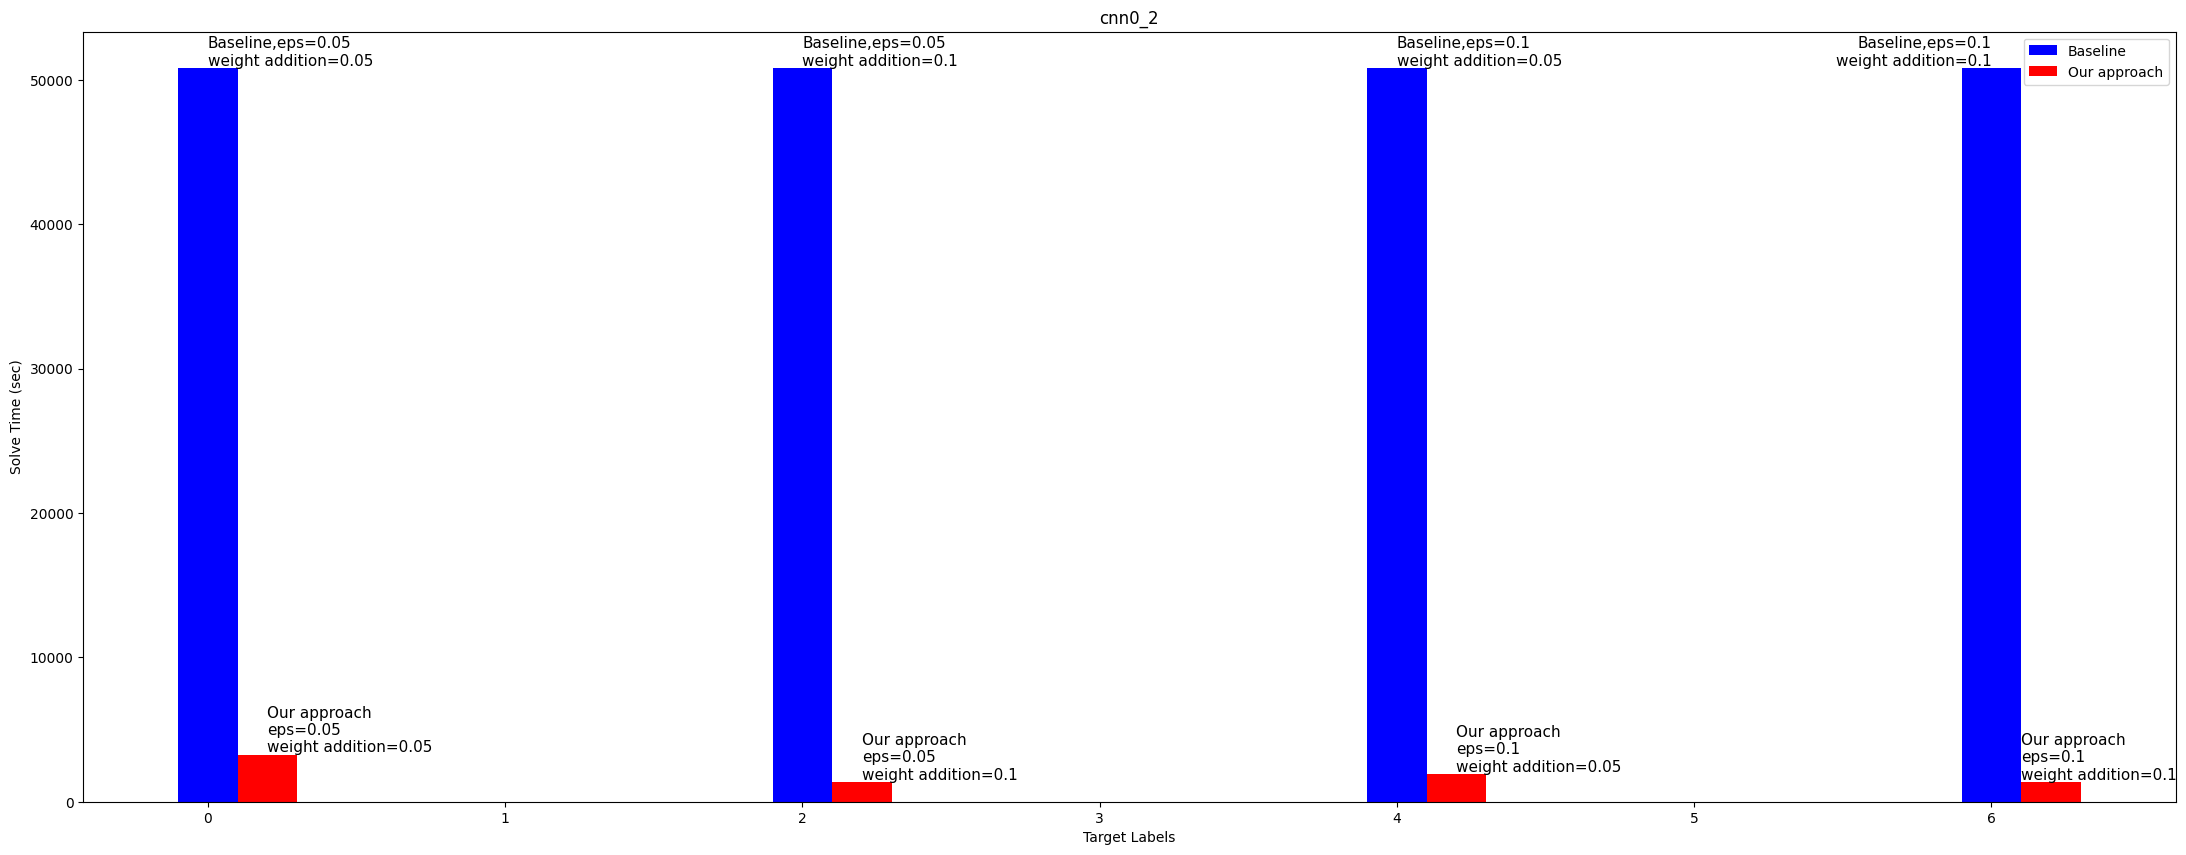
\includegraphics[width=0.95\textwidth]{cnn0_2.png}
  \caption{The execution time of the baseline against our approach, when the model type is a convolutional neural network, trained using 19 iterations .}
  \label{fig:cnn0_2}
\end{figure}


Table~\ref{table_3_x_10} shows that the bounds are slightly tighter when using the base approach, however it is negligible. Table~\ref{table_cnn0_1} and Table~\ref{table_cnn0_2} show better results when using our approach. This is due to timeout. the base approach is much slower, and does not manage to find tighter bound for more complex architectures before reaching timeout. Therefore, our approach enhances scalability and its accuracy is similar to the base approach for the tested scenario of two almost identical networks, besides a singular weight. Our goal is to further extend this improvement to other scenarios as well. 

\begin{table}[H]
	\centering
    \resizebox{\textwidth}{!}{
	\begin{tabular}{@{\extracolsep{\fill}}llllll@{}}
		\toprule
		& \makecell{ } & \makecell{Brightness[0.1] \\ Weight addition[0.1]} & \makecell{Brightness[0.1] \\ Weight addition[0.05]} & \makecell{Brightness [0.05] \\ Weight addition[0.1]} & \makecell{Brightness [0.05] \\ Weight addition[0.05]}\\
		\midrule			
		\multirow{2}{*}{Base approach} & upper bound  & 3.27 & 3.3 &  1.79 & 1.79\\
                              & lower bound & 3.27 & 3.27 &  1.79 & 1.79\\
		\midrule
		\multirow{2}{*}{Our approach} & upper bound  & 3.3 & 3.3 & 1.8 & 1.79\\
                              & lower bound & 3.27 & 3.27 & 1.79 & 1.79\\						
		\bottomrule
	\end{tabular}
}
\caption{The lower and upper bounds for 3X10 architecture 
		\label{table_3_x_10}}
\end{table}


\begin{table}[H]
	\centering
    \resizebox{\textwidth}{!}{
	\begin{tabular}{@{\extracolsep{\fill}}llllll@{}}
		\toprule
		& \makecell{ } & \makecell{Brightness[0.1] \\ Weight addition[0.1]} & \makecell{Brightness[0.1] \\ Weight addition[0.05]} & \makecell{Brightness [0.05] \\ Weight addition[0.1]} & \makecell{Brightness [0.05] \\ Weight addition[0.05]}\\
		\midrule			
		\multirow{2}{*}{Base approach} & upper bound  & 19.39 & 17.79 & 15.45 & 19.27\\
                              & lower bound & 15.01 & 15.01 &  12.18 & 12.19\\
		\midrule
		\multirow{2}{*}{Our approach} & upper bound  & 15.16 & 15.15 & 12.59 & 12.59\\
                              & lower bound & 15.01 & 15.01 &  12.46 & 12.46\\					
		\bottomrule
	\end{tabular}
}
\caption{The lower and upper bounds for CNN architecture with 20 iteration during training process.
		\label{table_cnn0_1}}
\end{table}


\begin{table}[H]
	\centering
    \resizebox{\textwidth}{!}{
	\begin{tabular}{@{\extracolsep{\fill}}llllll@{}}
		\toprule
		& \makecell{ } & \makecell{Brightness[0.1] \\ Weight addition[0.1]} & \makecell{Brightness[0.1] \\ Weight addition[0.05]} & \makecell{Brightness [0.05] \\ Weight addition[0.1]} & \makecell{Brightness [0.05] \\ Weight addition[0.05]}\\
		\midrule			
		\multirow{2}{*}{Base approach} & upper bound  & 15.77 & 17.71 & 15.6 & 19.16\\
                              & lower bound & 14.18 & 14.18 & 11.81 & 11.73\\
		\midrule
		\multirow{2}{*}{Our approach} & upper bound & 14.29 & 14.31 & 11.92 & 11.92\\
                              & lower bound & 14.15 & 14.17 & 11.8 & 11.81\\				
		\bottomrule
	\end{tabular}
}
\caption{The lower and upper bounds for CNN architecture with 19 iteration during training process.
		\label{table_cnn0_2}}
\end{table}
% NETA - image of database + explain: "hey we did good - but not good enough". 

% bounds in table
% times show in graph 